\documentclass[tikz,border=10pt]{standalone}
\usetikzlibrary{calc}

\begin{document}
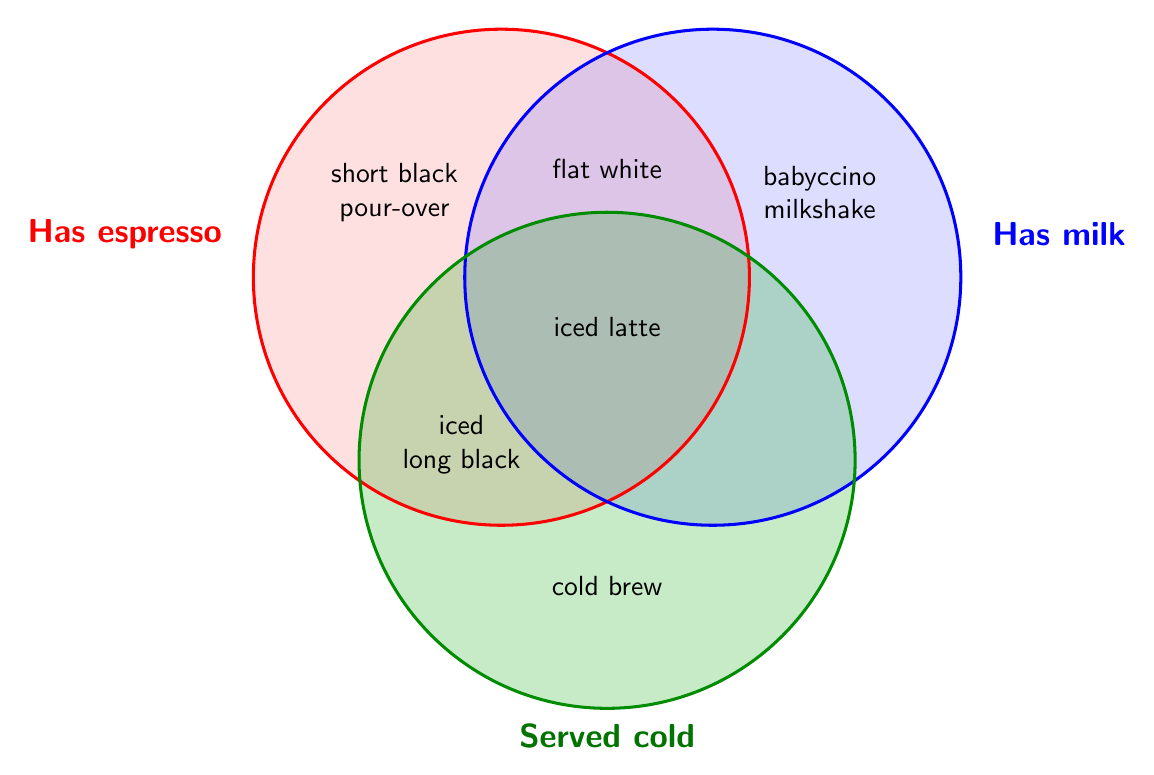
\begin{tikzpicture}[
  font=\sffamily,
  every node/.style={inner sep=0pt, outer sep=0pt},
  setlabel/.style={font=\sffamily\bfseries\large, align=center},
  item/.style={font=\sffamily, align=center}
]

% Equilateral centres, radius large enough that every overlap is a real region.
\def\R{3.15}
\coordinate (E) at (150:1.55);
\coordinate (M) at (30:1.55);
\coordinate (C) at (270:1.55);

\fill[red!55,   fill opacity=0.22] (E) circle (\R);
\fill[blue!60,  fill opacity=0.22] (M) circle (\R);
\fill[green!65!black, fill opacity=0.22] (C) circle (\R);

\draw[red,   line width=1.1pt] (E) circle (\R);
\draw[blue,  line width=1.1pt] (M) circle (\R);
\draw[green!55!black, line width=1.1pt] (C) circle (\R);

% Names sit outside the circles, not on the boundary.
\node[setlabel, red, anchor=east]  at ($(E)+(-3.55,0.55)$) {Has espresso};
\node[setlabel, blue, anchor=west] at ($(M)+( 3.55,0.55)$) {Has milk};
\node[setlabel, green!45!black, anchor=north] at ($(C)+(0,-3.35)$) {Served cold};

% Espresso only (hot, no milk)
\node[item] at (-2.70, 1.85) {short black\\pour-over};
% Milk only (not espresso, not cold)
\node[item] at ( 2.70, 1.85) {babyccino\\milkshake};
% Cold only (no espresso, no milk)
\node[item] at ( 0.00,-3.15) {cold brew};

% Espresso and milk, served hot
\node[item] at ( 0.00, 2.15) {flat white};
% Espresso, cold, no milk
\node[item] at (-1.85,-1.35) {iced\\long black};
% Espresso, milk, and cold
\node[item] at ( 0.00, 0.15) {iced latte};

% Milk and cold, but no espresso: none of the listed drinks.

\end{tikzpicture}
\end{document}
